\documentclass[a4paper,11pt]{article}
%\pdfoutput=1 % if your are submitting a pdflatex (i.e. if you have
             % images in pdf, png or jpg format)
\usepackage{jheppub} % for details on the use of the package, please
                     % see the JHEP-author-manual
\usepackage[T1]{fontenc} % if needed

\usepackage{slashed}
%\usepackage{subfigure}
\usepackage{xspace}
\usepackage{booktabs}
%% %simple case: 2 authors, same institution
%% \author{A. Uthor}
%% \author{and A. Nother Author}
%% \affiliation{Institution,\\Address, Country}


\title{Electroweak corrections with MadDM v.3.0}

\author[a]{Federico Ambrogi}
\affiliation[a]{University of Vienna, Faculty of Physics, Bolzmanngasse 5, A-1090 Wien, Austria}
% e-mail addresses: one for each author, in the same order as the authors\emailAdd{federico.ambrogi@oeaw.ac.at}
\emailAdd{federico.ambrogi88@gmail.com}


%%% Various Tools
\newcommand{\amc}{{\sc MadGraph5\textunderscore}a{\sc MC@NLO}}
\newcommand{\pyE}{{\sc Pythia\,8}\xspace}

\newcommand{\PPPC}{\texttt{PPPC4DMID}}
\newcommand{\PPPCew}{\texttt{PPPC4DMID\_ew}}

\newcommand{\MADDM}{\texttt{MadDM v.3.0}}


\abstract{{\color{blue} This documents summarises the status of the studies of the discrepancies found in the energy spectra provided in the \PPPC tables and the spectra produced with \MADDM, when considering electro weak corrections.} }      

\begin{document} 
\sffamily
\maketitle
\flushbottom
\section{PPPC Electroweak Corrections}
In this section the energy spectra for the Cosmic Rays $CRs = e^+, \nu_e , \gamma$ extracted from the \PPPC and \PPPCew Tables are compared, to get an idea of the effect of the EW correction (according the \PPPC collaboration). 

\begin{figure}[!]
\begin{center}
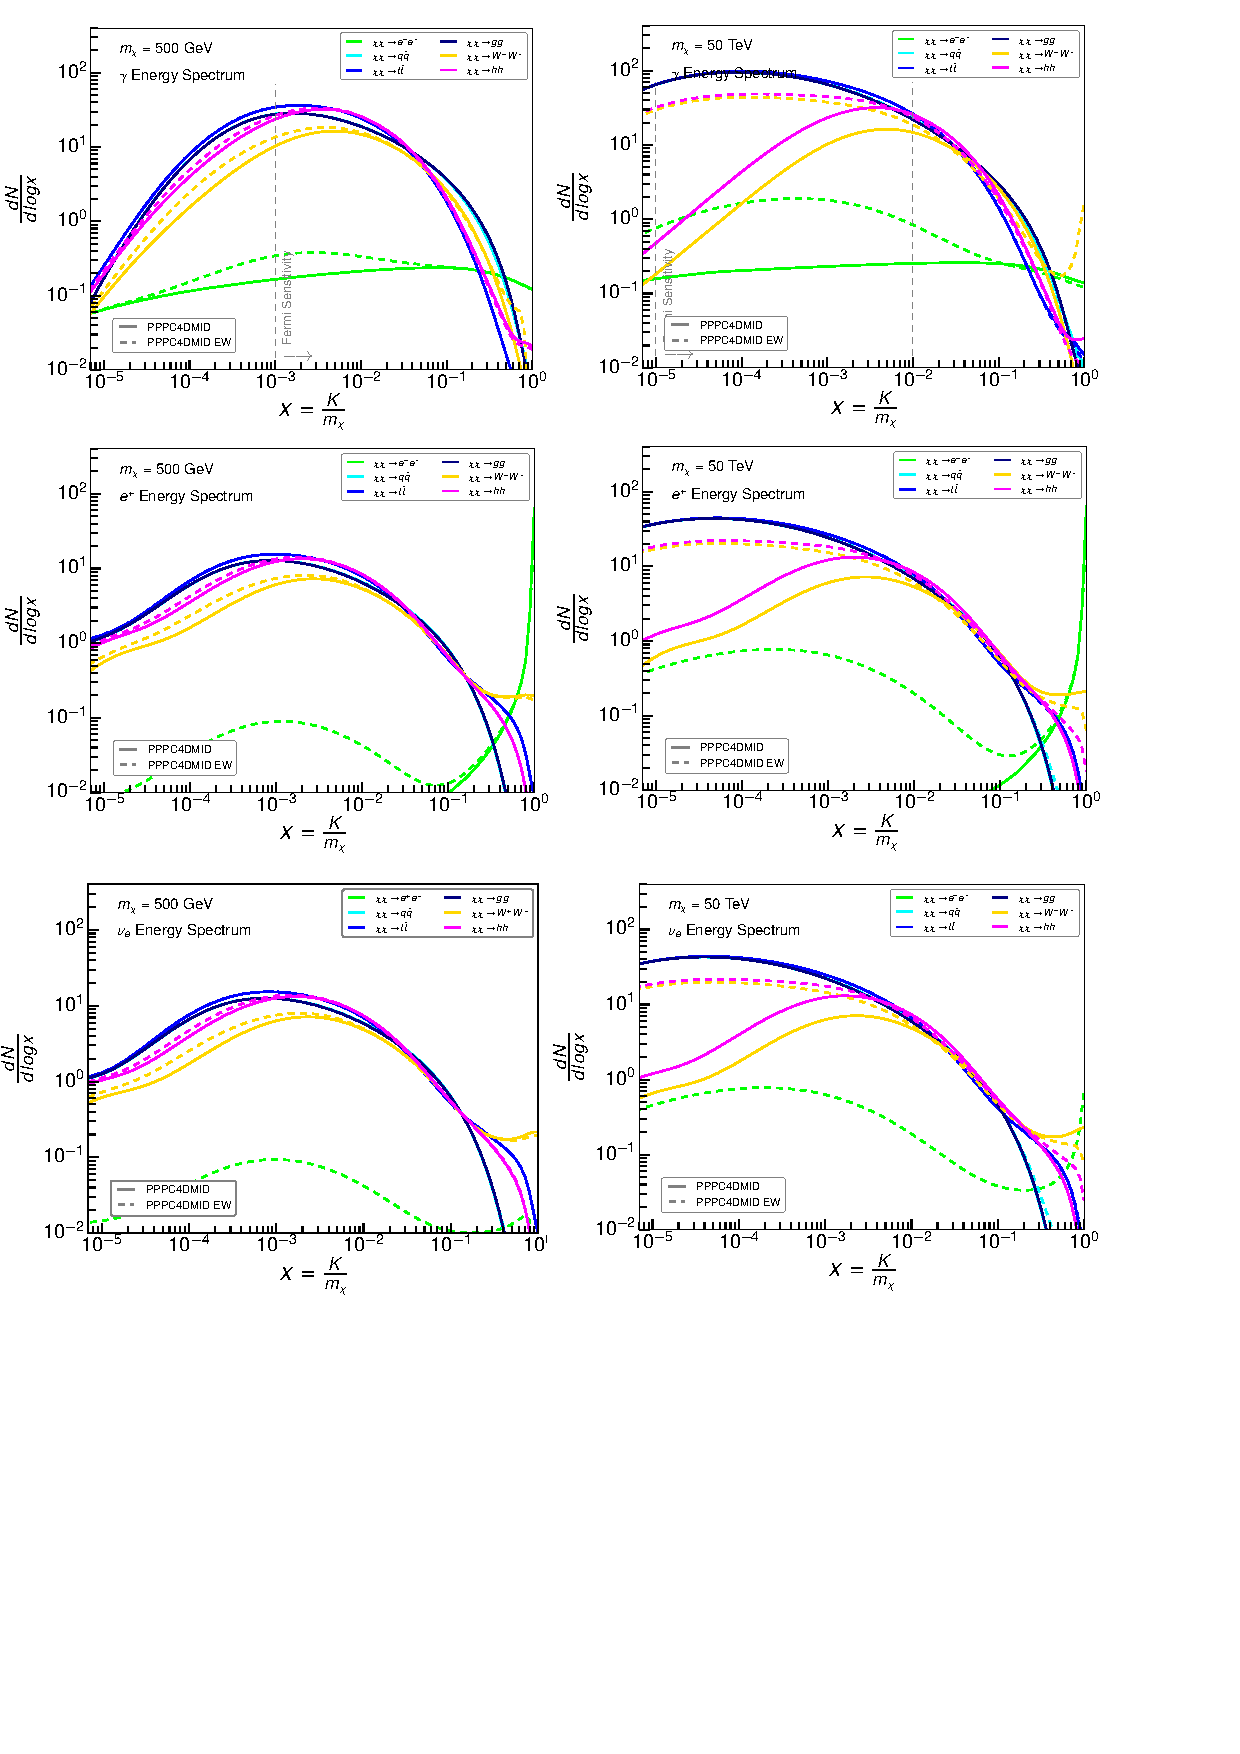
\includegraphics[width=1\textwidth]{Fig/EW_noEW_PPPC.pdf}
\end{center}
\caption{Energy spectra ($\gamma, \e^+, \nu_e$) for $m_{\chi}=$500 GeV (left) and 50 TeV (right) extracted from the \PPPC and \PPPCew tables, from selected annihilation channels.}
\end{figure}





\section{MadDM vs PPPC Electroweak Corrections}

\begin{figure}[!]
\begin{center}
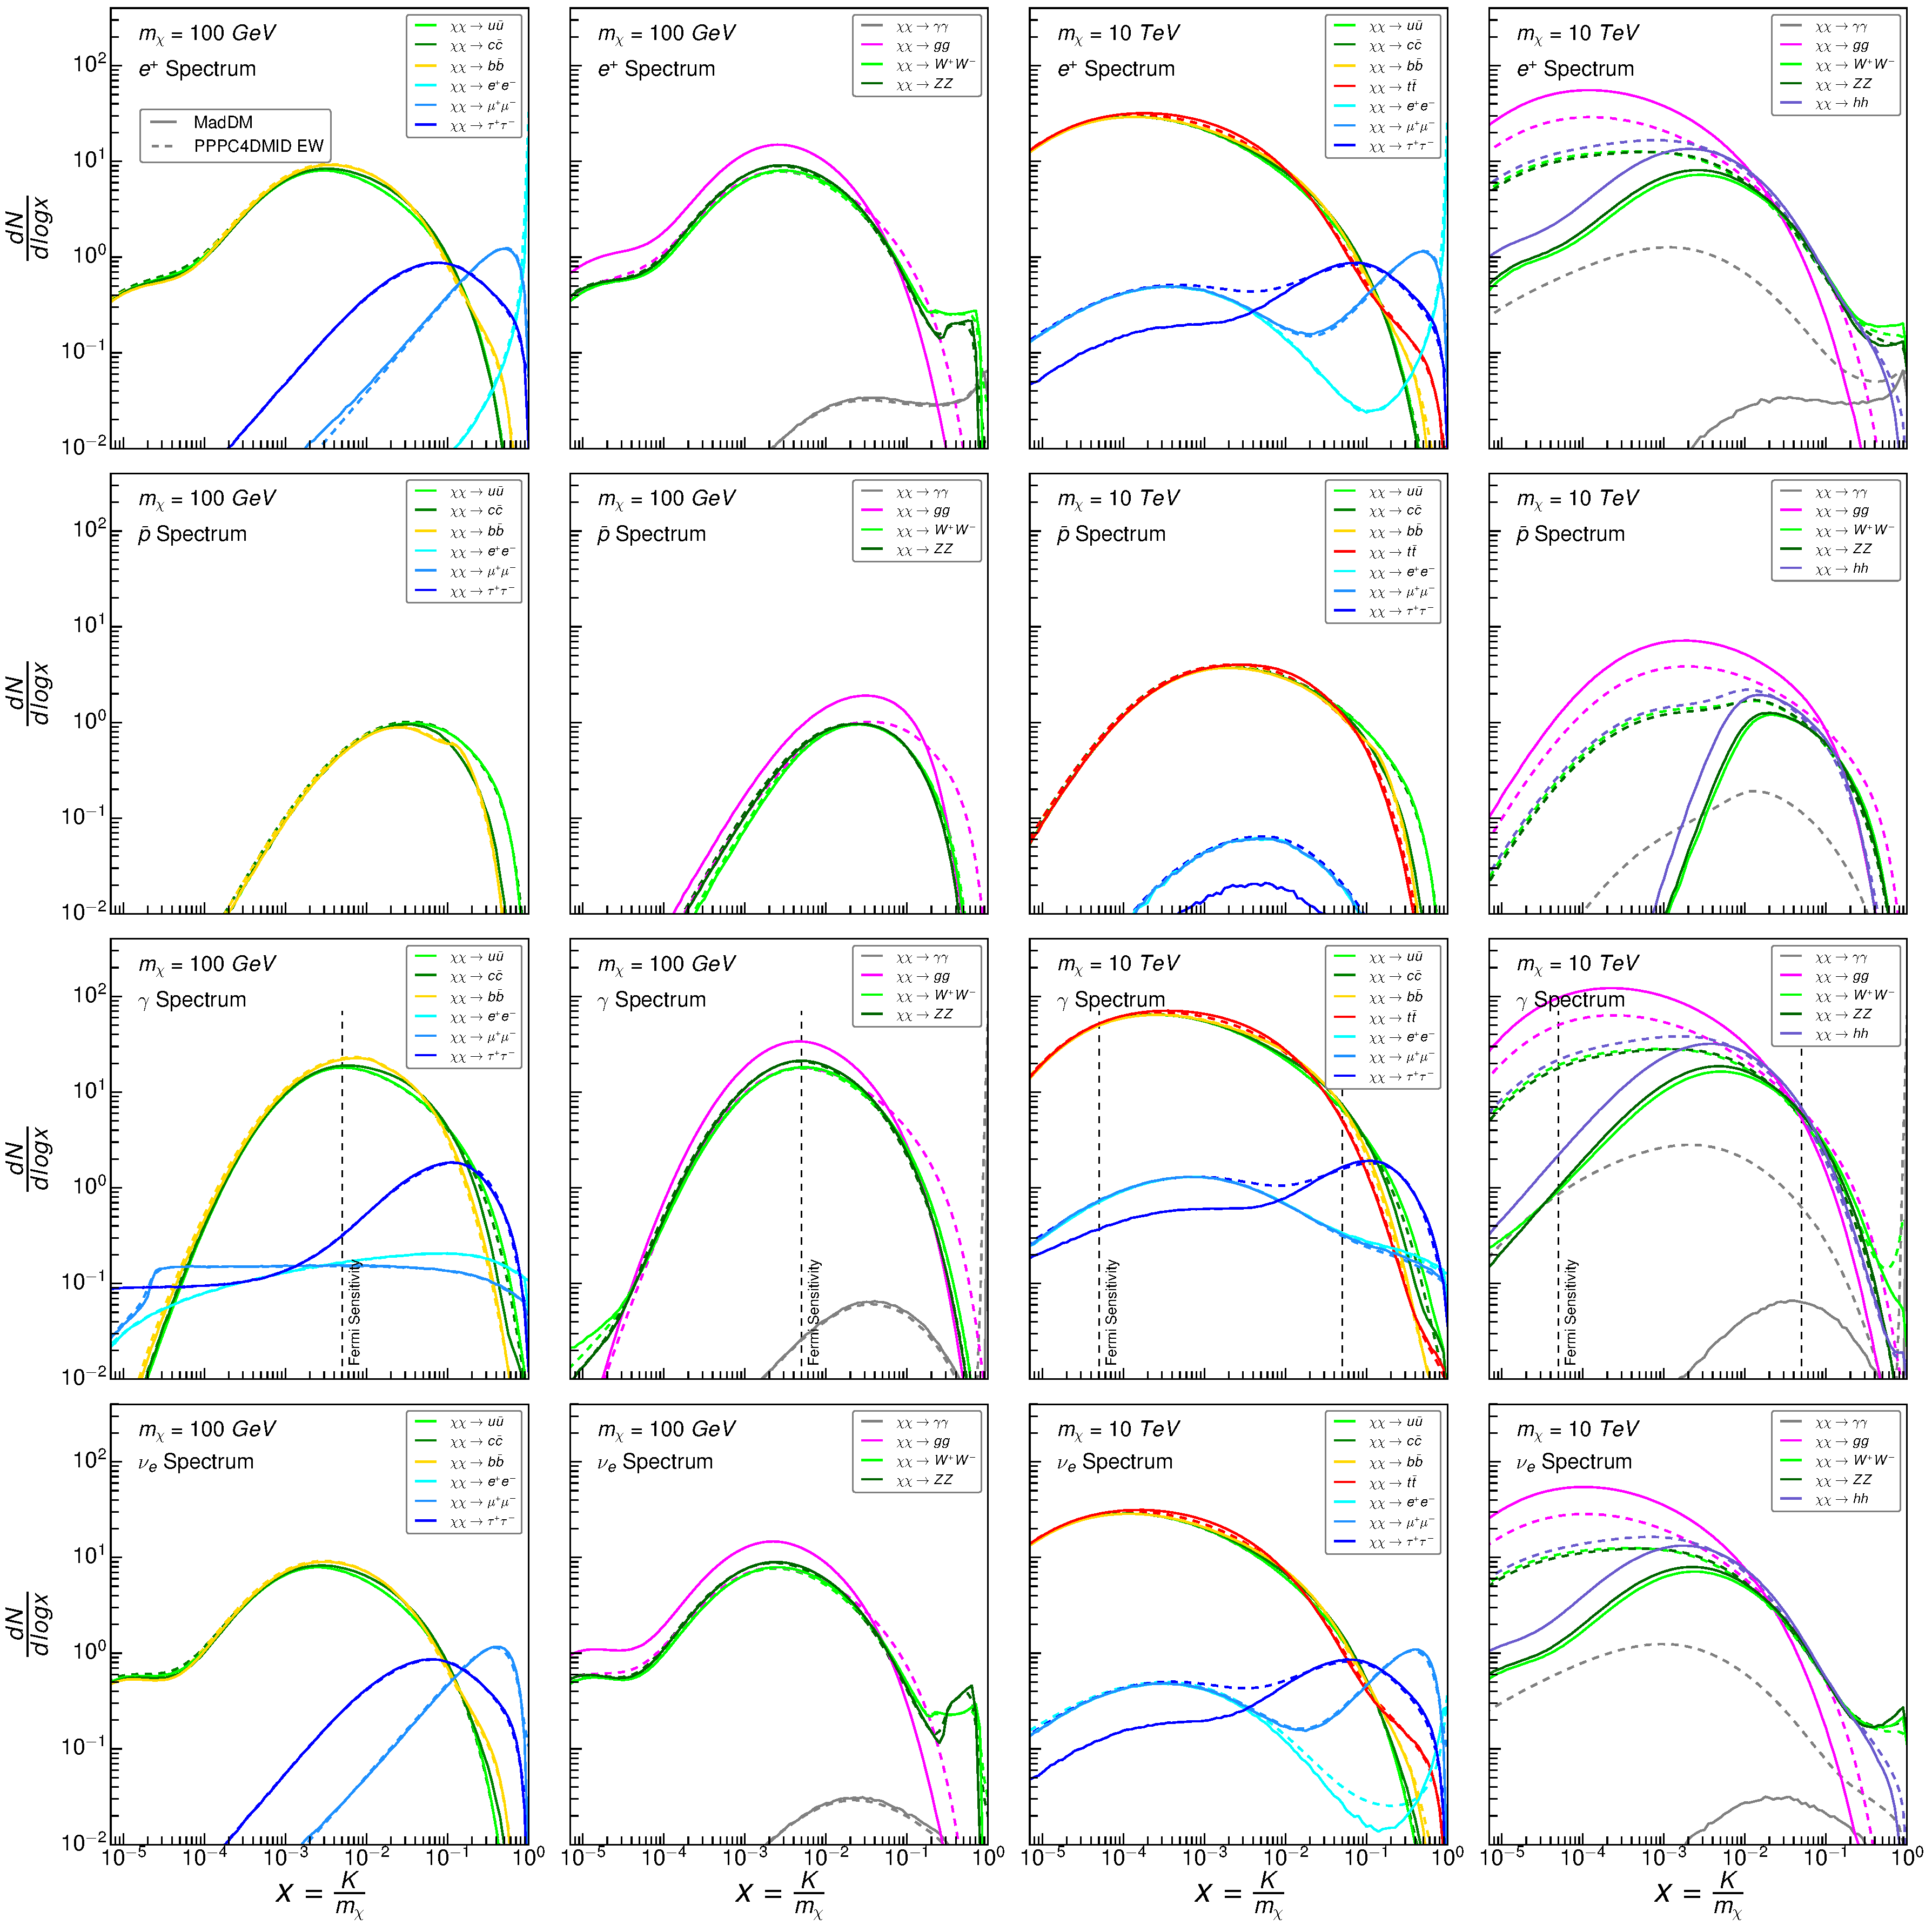
\includegraphics[width=1\textwidth]{Fig/EW_Grid_Plots.pdf}
\end{center}
\caption{EW Spectra comparison \MADDM vs \PPPCew (published in the paper).}
\end{figure}





\section*{Acknowledgments}





\bibliographystyle{JHEP}
\bibliography{references}


\end{document}
